
\subsection{Hardware - V2.2}
\setAuthor{Richard Krammer}

    This section describes the latest hardware of the basic node. The basic node is a 
    simple node that can measure the ambient temperature and control four RGB-LEDs.
    The hardware consists of the following components:

    \begin{itemize}
        \item Microcontroller
        \item Temperature sensor
        \item LED Indicator
        \item USB-C Connector
        \item 3.3V DC-DC Converter
        \item Module-Connector
    \end{itemize}

    \subsubsection{Microcontroller}
        The basic node uses an ESP32 C3 microcontroller. It is a low-power, highly
        integrated Wi-Fi and Bluetooth SoC. In the datasheet it was stated that the
        MCU is recommended for a wide range of applications, including smart home devices 
        and other IoT products.

        \begin{figure}[H]
            \centering
            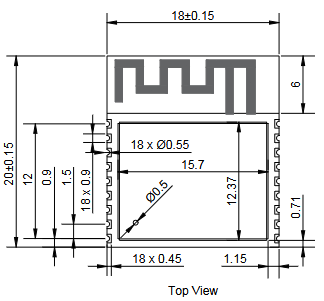
\includegraphics[width=0.7\textwidth]{assets/HW/ESP32-C3-sheet.png}
            \caption{ESP-C3 Datasheet in mm}
        \end{figure}

    
    \subsubsection{Temperature sensor}
        The DS18B20 was chosen as the temperature sensor. It is a digital thermometer
        with an operating temperature range of -55°C to +125°C. The sensor is connected
        to the microcontroller via GPIO0 and communicates over a 1-Wire bus.
        It is fairly compact and would not take up much space on the PCB.

        \begin{figure}[H]
            \centering
            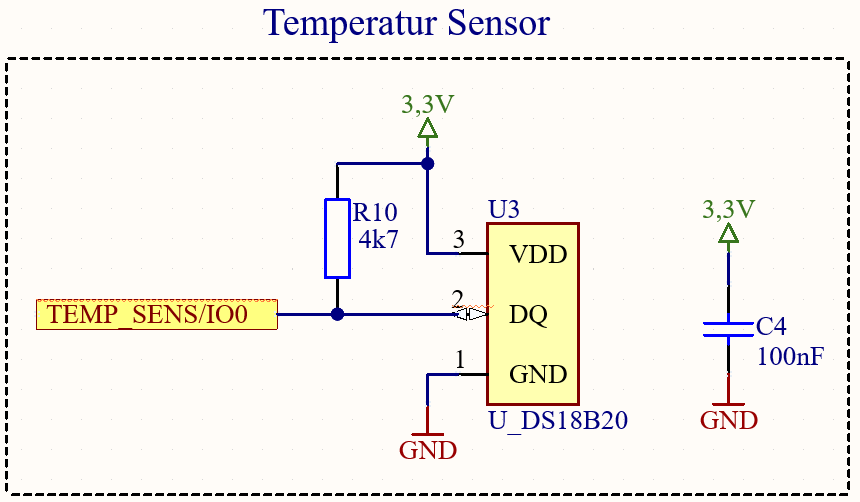
\includegraphics[width=0.7\textwidth]{assets/HW/DS18B20-schematic.png}
            \caption{DS18B20 implemented in the schematic.}
        \end{figure}

    \subsubsection{LED Indicator}
        The basic node has four WS2813b ARGB-LEDs. The LEDs are connected to the 
        microcontroller via GPIO 2. The LEDs are used to indicate the status of the node. 
        For example, the LEDs can be used to indicate the temperature range the node is in
        or to display the charge-level of the battery, when attached.

        \begin{figure}[H]
            \centering
            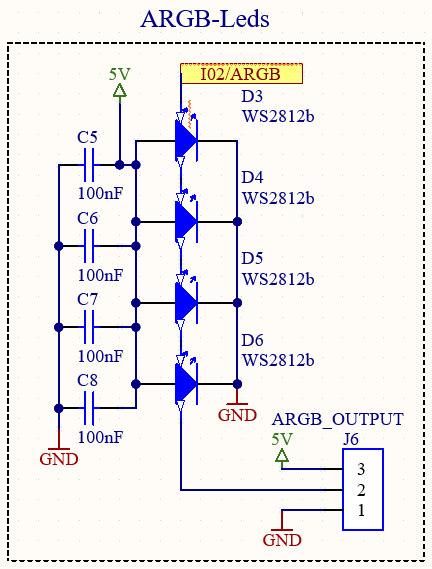
\includegraphics[width=0.7\textwidth]{assets/HW/RGB-LED-schematic.png}
            \caption{RGB-LEDs implemented in the schematic.}
        \end{figure}

    \subsubsection{USB-C Connector}

    \subsubsection{3.3V DC-DC Converter}

    \subsubsection{Module-Connector}

\subsection{Hardware - V2.1}

\subsection{Hardware - V2.0}

\subsection{Hardware - V1.0}
        